
%(BEGIN_QUESTION)
% Copyright 2010, Tony R. Kuphaldt, released under the Creative Commons Attribution License (v 1.0)
% This means you may do almost anything with this work of mine, so long as you give me proper credit

Suppose the lamp refuses to light up when the pushbutton switch is pressed.  A voltmeter registers 0 volts between test points {\bf A} and {\bf D} in the circuit while the pushbutton is pressed:

$$\includegraphics[width=15.5cm]{i01555x01.eps}$$

Determine the diagnostic value of each of the following tests.  Assume only one fault in the system, including any single component or any single wire/cable/tube connecting components together.  If a proposed test could provide new information to help you identify the location and/or nature of the one fault, mark ``yes.''  Otherwise, if a proposed test would not reveal anything relevant to identifying the fault (already discernible from the measurements and symptoms given so far), mark ``no.''

% No blank lines allowed between lines of an \halign structure!
% I use comments (%) instead, so that TeX doesn't choke.

$$\vbox{\offinterlineskip
\halign{\strut
\vrule \quad\hfil # \ \hfil & 
\vrule \quad\hfil # \ \hfil & 
\vrule \quad\hfil # \ \hfil \vrule \cr
\noalign{\hrule}
%
% First row
{\bf Diagnostic test} & {\bf Yes} & {\bf No} \cr
%
\noalign{\hrule}
%
% Another row
Measure $V_{EF}$ with switch pressed &  &  \cr
%
\noalign{\hrule}
%
% Another row
Measure $V_{CD}$ with switch pressed &  &  \cr
%
\noalign{\hrule}
%
% Another row
Measure $V_{CB}$ with switch pressed &  &  \cr
%
\noalign{\hrule}
%
% Another row
Measure $V_{CE}$ with switch pressed &  &  \cr
%
\noalign{\hrule}
%
% Another row
Measure $R_{AB}$ with switch pressed &  &  \cr
%
\noalign{\hrule}
%
% Another row
Measure $V_{EF}$ with switch unpressed &  &  \cr
%
\noalign{\hrule}
%
% Another row
Measure $V_{CD}$ with switch unpressed &  &  \cr
%
\noalign{\hrule}
%
% Another row
Measure $V_{CB}$ with switch unpressed &  &  \cr
%
\noalign{\hrule}
%
% Another row
Measure $V_{CE}$ with switch unpressed &  &  \cr
%
\noalign{\hrule}
%
% Another row
Measure $R_{AB}$ with switch unpressed &  &  \cr
%
\noalign{\hrule}
} % End of \halign 
}$$ % End of \vbox

\vfil 

\underbar{file i01555}
\eject
%(END_QUESTION)





%(BEGIN_ANSWER)

% No blank lines allowed between lines of an \halign structure!
% I use comments (%) instead, so that TeX doesn't choke.

$$\vbox{\offinterlineskip
\halign{\strut
\vrule \quad\hfil # \ \hfil & 
\vrule \quad\hfil # \ \hfil & 
\vrule \quad\hfil # \ \hfil \vrule \cr
\noalign{\hrule}
%
% First row
{\bf Diagnostic test} & {\bf Yes} & {\bf No} \cr
%
\noalign{\hrule}
%
% Another row
Measure $V_{EF}$ with switch pressed & $\surd$ &  \cr
%
\noalign{\hrule}
%
% Another row
Measure $V_{CD}$ with switch pressed & $\surd$ &  \cr
%
\noalign{\hrule}
%
% Another row
Measure $V_{CB}$ with switch pressed & $\surd$ &  \cr
%
\noalign{\hrule}
%
% Another row
Measure $V_{CE}$ with switch pressed & $\surd$ &  \cr
%
\noalign{\hrule}
%
% Another row
Measure $R_{AB}$ with switch pressed & $\surd$ &  \cr
%
\noalign{\hrule}
%
% Another row
Measure $V_{EF}$ with switch unpressed & $\surd$ &  \cr
%
\noalign{\hrule}
%
% Another row
Measure $V_{CD}$ with switch unpressed &  & $\surd$ \cr
%
\noalign{\hrule}
%
% Another row
Measure $V_{CB}$ with switch unpressed &  & $\surd$ \cr
%
\noalign{\hrule}
%
% Another row
Measure $V_{CE}$ with switch unpressed & $\surd$ &  \cr
%
\noalign{\hrule}
%
% Another row
Measure $R_{AB}$ with switch unpressed & $\surd$ &  \cr
%
\noalign{\hrule}
} % End of \halign 
}$$ % End of \vbox

%(END_ANSWER)





%(BEGIN_NOTES)


%INDEX% Troubleshooting review: electric circuit diagnostic test usefulness

%(END_NOTES)


